\section{Тестирование системы}

\subsection{Условия и порядок тестирования}

Объектом тестирования является портал подрядных организаций.

При каждом построении исполняемого модуля информационной системы происходит тестирование представлений на предмет ошибок времени исполнения.
Такой вид тестирования называется теневым, так как не предполагает каких-либо исходных данных.
Данный метод был реализован при помощи развёртывания сервера автоматического построения проектов TeamCity.

Нагрузочное тестирование предполагает собой проверку на максимальное число соединений или запросов от клиентов информационной системы, при котором последняя корректно функционирует.
Под корректным функционированием в данном случае принимается работа информационной системы без возникновения исключельных ситуаций при верно введённых данных.
Данное тестирование выполняется раз в месяц при помощи средств, представленных инструментальной средой разработки и платформой, на которой ведётся разработка информационной системы.

Для проверки графического интерфейса пользователя используются средства создания снимков веб-страниц.
К ним можно отнести такие программы как SlimerJS и PhantomJS.
Данные средства позволяют выполнять сценарии прохождения пользователя по сайту (симулируется работа реального пользователя).
На каждом шаге можно сделать снимок страницы и сохранить его в файловую систему.

\subsection{Исходные данные для контрольных примеров}

%\subsubsection*{Нагрузочное тестирование}
Для нагрузочного тестирования было выбрано три страницы:

\begin{enumerate}
	\item главная страница;
	\item список конкурсов;
	\item подробности конкурса;
\end{enumerate}

Был составлен тест, при котором эмулируется работа пятидесяти пользователей одновременно в течение десяти минут.
Эти пользователи последостельно заходят на каждую тестируемую страницу с определёнными временными задержками.
Испытание считается пройденным, если страница с её зависимостями загрузилась за минуту.
Изменяется число обработанных запросов в секунду, а также задержки при загрузке страниц.

%\subsubsection*{Проверка графического интерфейса}
Для тестирования графического интерфейса площадки подрядчиков была написана утилита на основе технологии SlimerJs для создания снимков экрана основных страниц сайта.
Её исходный текст представлен в приложении~В.

\subsection{Результаты тестирования}

Результаты теневого тестирования показали, что все представления, используемые в информационной системе, не содержат неверной разметки, что может повлиять на отображение информации в различных приложениях-браузерах.

Результаты нагрузочного тестирования показали, что система справляется с нагрузкой в 50 человек.

Число загруженных страниц в секунду представлено в графике на рисунке~\ref{img:test-pagespersec}.

\begin{figure}[h!]
	\begin{center}
		\begin{minipage}[h]{\linewidth}
			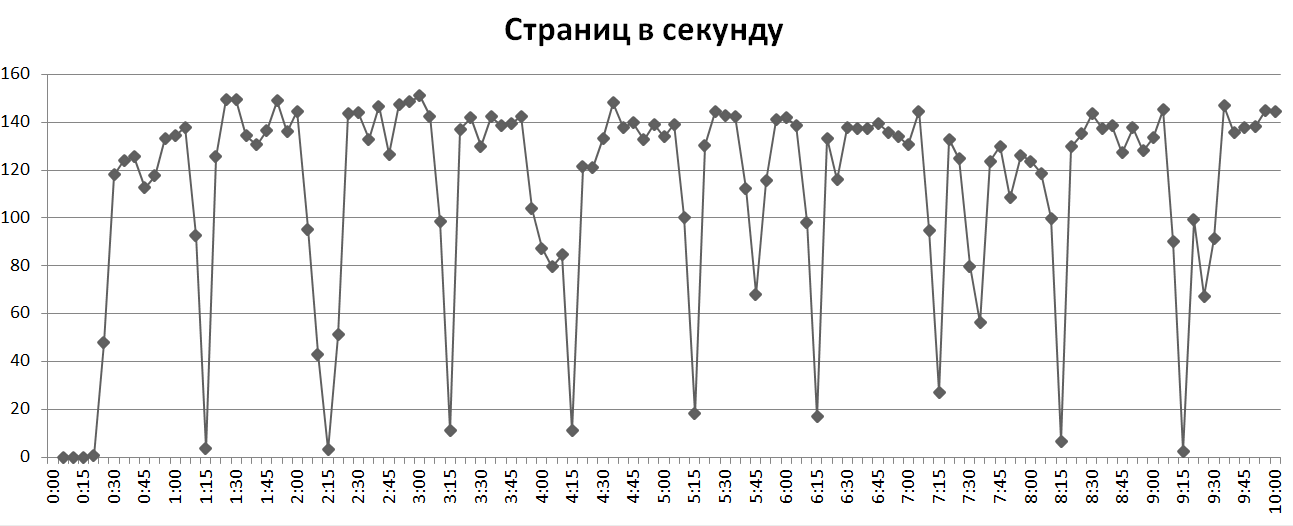
\includegraphics[width=\linewidth]{images/test-pagespersec.png}
			\caption{Число загруженных страниц в секунду}
			\label{img:test-pagespersec}
		\end{minipage}
		\hfill
	\end{center}
\end{figure}

Как можно видеть, среднее число загруженных страниц находится в пределах от 120 до 150 страниц.
Примерно раз в минуту имеет место быть деградация значения до 10 страниц в секуду.
Скорее всего, это связано с сбросом кеш-памяти либо у сервера, либо у клиента.
Такие отклонения незначительны и не могут кардинально нарушить работу системы.

Время загрузки страниц в секундах представлено в графике на рисунке~\ref{img:test-loadingtime}.

\begin{figure}[h!]
	\begin{center}
		\begin{minipage}[h]{\linewidth}
			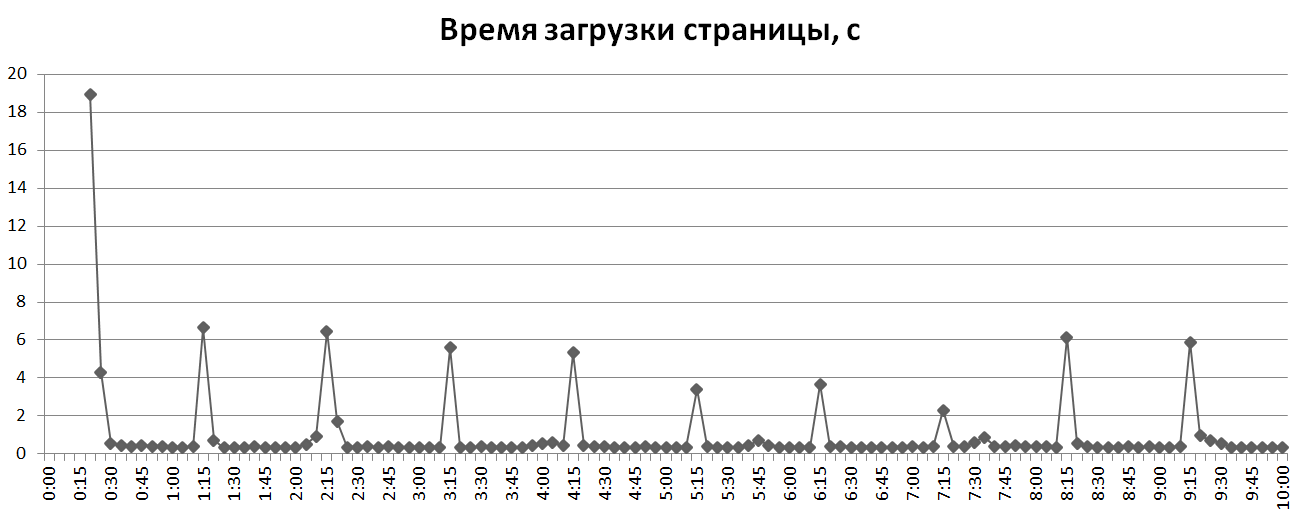
\includegraphics[width=\linewidth]{images/test-loadingtime.png}
			\caption{Среднее время загрузки страницы}
			\label{img:test-loadingtime}
		\end{minipage}
		\hfill
	\end{center}
\end{figure}

Как можно заметить, в подавляющем большинстве случаев среднее время загрузки страницы не превышает двух секунд.
Однако встречаются значения выше четырёх секунд.
Это происходит примерно раз в минуту.
Причина этих пиков также, скорее всего, связана с кешированием данных.

Общие результаты тестирования представлены в таблице~\ref{tab:test-results}.

\begin{footnotesize}
\begin{longtable}[h]{|p{0.05\textwidth}|p{0.7\textwidth}|p{0.15\textwidth}|}
	\caption{\label{tab:test-results}Результаты нагрузочного тестирования системы} \\
	\hline
		\thead{№} & \thead{Параметр} & \thead{Значение} \\
	\hline
		\theadnum{1} & \theadnum{2} & \theadnum{3} \\
	\hline \endfirsthead
	\hline
		 \theadnum{1} & \theadnum{2} & \theadnum{3} \\
	\hline \endhead
	1 & Число пользователей одновременно & 50 \\ \hline
	2 & Тестов в секунду & 37,3 \\ \hline
	3 & Тестов провалено & 0 \\ \hline
	4 & Среднее время выполнение теста в секундах & 1,34 \\ \hline
	5 & Страниц в секунду & 112 \\ \hline
	6 & Среднее время загрузки страницы в секундах & 0,44 \\ \hline
	7 & Запросов в секунду & 572 \\ \hline
	8 & Запросов заблокировано & 0 \\ \hline
	9 & Процент закешированных запросов & 74,2 \\ \hline
	10 & Среднее время ответа в секундах & 0,11 \\ \hline
	11 & Средняя длина ответа в байтах & 5419 \\ \hline
\end{longtable}
\end{footnotesize}

Тестом в данном случае считается обход трёх страниц, указанных в исходных данных на нагрузочное тестирование.

Как можно видеть из результатов, система быстро реагирует на запросы.
Ни одной ошибки не было возвращено, также как и ни один запрос не был заблокирован.

Результаты тестирования графического интерфейса пользователя показали, что все страницы портала подрядчиков корректно отображаются на устройствах с диагональю экрана более 4,7 дюйма.
Удобное для пользования системой разрешение экрана -- 1366х768 и выше.

Пример отображения списка конкурсов можно видеть на рисунке~\ref{img:test-smartphone}.
Снимок экрана был произведён с телефона LG D410 с диагональю 4.7 дюйма.

\begin{figure}[h!]
	\begin{center}
		\begin{minipage}[h]{\linewidth}
			\centering
			
\includegraphics[width=0.35\linewidth]{images/test-smartphone.png}
			\caption{Адаптивность дизайна под мобильные платформы}
			\label{img:test-smartphone}
		\end{minipage}
		\hfill
	\end{center}
\end{figure}

\clearpage
\newpage